\documentclass[tikz,border=10pt]{standalone}
% Figure: rectangle ABCD with bend point E and right-angle mark at E.
% Scale from STYLE METRICS: s = 0.019324 cm/px (longest side = 8 cm), centre (244,183) px.
\begin{document}
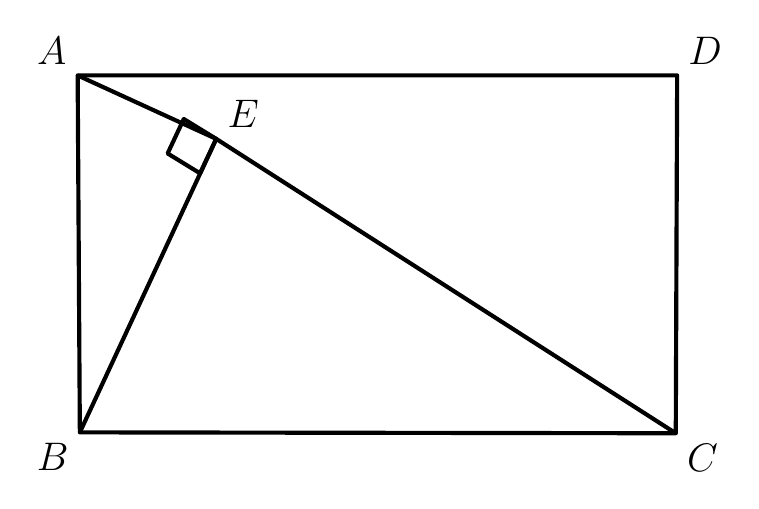
\begin{tikzpicture}[line join=round, line width=1.5pt]

% Named coordinates (x=(px-244)*s, y=(183-py)*s)
\coordinate (A) at (-3.8068, 2.2802);
\coordinate (D) at ( 3.8068, 2.2802);
\coordinate (C) at ( 3.7892,-2.2643);
\coordinate (B) at (-3.7790,-2.2529);
\coordinate (E) at (-2.0469, 1.4742);

% Right-angle square corners at E (from verified mark points)
\coordinate (P1) at (-2.4592, 1.7265);
\coordinate (P2) at (-2.6642, 1.2891);
\coordinate (P3) at (-2.2524, 1.0368);

% Rectangle sides: straight segments only
\draw (A) -- (D) -- (C) -- (B) -- cycle;

% A-E-C path: two straight segments (plain --, no curve/arc/bend)
\draw (A) -- (E) -- (C);

% Segment B-E: straight
\draw (B) -- (E);

% Right-angle mark at E (one square)
\draw (E) -- (P1) -- (P2) -- (P3) -- cycle;

% Labels (font from STYLE METRICS)
\node[above left,  font=\fontsize{15.5}{18.6}\selectfont] at (A) {$A$};
\node[above right, font=\fontsize{15.5}{18.6}\selectfont] at (D) {$D$};
\node[below left,  font=\fontsize{15.5}{18.6}\selectfont] at (B) {$B$};
\node[below right, font=\fontsize{15.5}{18.6}\selectfont] at (C) {$C$};
\node[above right, font=\fontsize{15.5}{18.6}\selectfont] at (E) {$E$};

\end{tikzpicture}
\end{document}